\documentclass[aspectratio=169, 11pt]{beamer}

% ── Theme ──
\usetheme{Madrid}
\usecolortheme{seahorse}
\setbeamertemplate{navigation symbols}{}
\setbeamertemplate{footline}{%
  \leavevmode\hbox{%
    \begin{beamercolorbox}[wd=.33\paperwidth,ht=2.5ex,dp=1ex,center]{author in head/foot}%
      \usebeamerfont{author in head/foot}\insertshortauthor
    \end{beamercolorbox}%
    \begin{beamercolorbox}[wd=.34\paperwidth,ht=2.5ex,dp=1ex,center]{title in head/foot}%
      \usebeamerfont{title in head/foot}\insertshorttitle
    \end{beamercolorbox}%
    \begin{beamercolorbox}[wd=.33\paperwidth,ht=2.5ex,dp=1ex,right]{date in head/foot}%
      \usebeamerfont{date in head/foot}\insertframenumber{} / \inserttotalframenumber\hspace*{2ex}
    \end{beamercolorbox}}%
}

\usepackage{amsmath,amssymb}
\usepackage{graphicx}
\usepackage{booktabs}
\usepackage{tikz}

% ── Meta ──
\title[2D Burgers' Mini-App]{Mini-App: 2D Viscous Burgers' Equation}
\subtitle{CS555: Numerical Methods for PDEs --- Spring 2026}
\author{Atharva \and Liza}
\newcommand{\profname}{Prof.\ Paul Fischer}
\institute{University of Illinois Urbana-Champaign}
\date{Spring 2026}

\begin{document}

% ============================================================
%  SLIDE 1 -- Title
% ============================================================
\begin{frame}
  \titlepage
  \centering\profname
\end{frame}

% ============================================================
%  SLIDE 2 -- Problem Statement & Motivation
% ============================================================
\begin{frame}{Problem Statement}
  \textbf{Goal:} Explore the interplay of advection and diffusion in numerical PDE solvers.

  \medskip
  The \textbf{2D coupled viscous Burgers' equations}:
  \begin{align*}
    u_t + u\,u_x + v\,u_y &= \nu\,(u_{xx} + u_{yy}) \\
    v_t + u\,v_x + v\,v_y &= \nu\,(v_{xx} + v_{yy})
  \end{align*}

  \begin{itemize}
    \item Nonlinear advection (hyperbolic) $+$ linear diffusion (parabolic)
    \item \textbf{Cole--Hopf transformation} provides an exact solution for verification
    \item Domain: $[0,1]^2$, Dirichlet BCs from the exact solution
    \item Reynolds number $\mathrm{Re} = UL/\nu$ controls solution sharpness
  \end{itemize}

  \medskip
  \textbf{Mini-app highlights:}
  Convergence rates, stability limits, cost trade-offs, and viscosity effects.
\end{frame}

% ============================================================
%  SLIDE 3 -- Implementation Overview
% ============================================================
\begin{frame}{Implementation Overview}
  \begin{columns}[T]
    \begin{column}{0.48\textwidth}
      \textbf{Spatial Discretization}
      \begin{itemize}
        \item Central differences ($O(h^2)$)
        \item First-order upwind ($O(h)$)
        \item Laplacian via Kronecker products
      \end{itemize}

      \bigskip
      \textbf{Temporal Discretization}
      \begin{itemize}
        \item Forward Euler --- $O(\Delta t)$
        \item RK4 --- $O(\Delta t^4)$
        \item Backward Euler (semi-implicit) --- $O(\Delta t)$
        \item Crank--Nicolson with predictor-corrector --- $O(\Delta t^2)$
      \end{itemize}
    \end{column}

    \begin{column}{0.48\textwidth}
      \textbf{Key Design Choices}
      \begin{itemize}
        \item Built from first principles in Python
        \item Implicit methods: sparse LU factorization (pre-factored once)
        \item RK4 CFL monitoring: tracks both advective and diffusive limits
        \item Cole--Hopf exact solution for rigorous error measurement
      \end{itemize}

      \bigskip
      \textbf{Verification Strategy}
      \begin{itemize}
        \item Discrete $L^2$ and $L^\infty$ norms
        \item Spatial \& temporal convergence studies
        \item Stability boundary probes
      \end{itemize}
    \end{column}
  \end{columns}
\end{frame}

% ============================================================
%  SLIDE 4 -- Reference Solution
% ============================================================
\begin{frame}{Reference Solution ($\nu = 0.01$, $\mathrm{Re} \approx 100$, $T = 0.5$)}
  \begin{columns}[c]
    \begin{column}{0.50\textwidth}
      \centering
      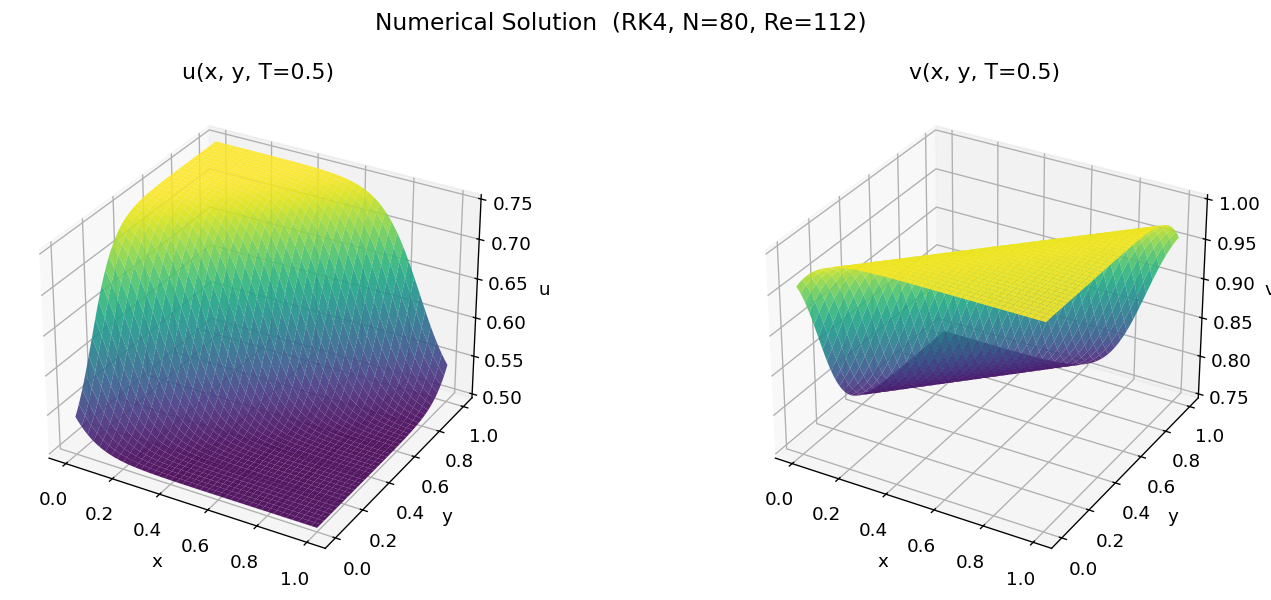
\includegraphics[width=\textwidth]{figures/fig_01_cell10.png}
    \end{column}
    \begin{column}{0.48\textwidth}
      \begin{itemize}
        \item $81 \times 81$ grid, RK4, $\Delta t = 10^{-4}$
        \item Diagonal front from Cole--Hopf solution
        \item $L^2$ error $\sim 10^{-5}$
        \item Solution verified against exact Cole--Hopf
      \end{itemize}
      \vspace{-2pt}
      \centering
      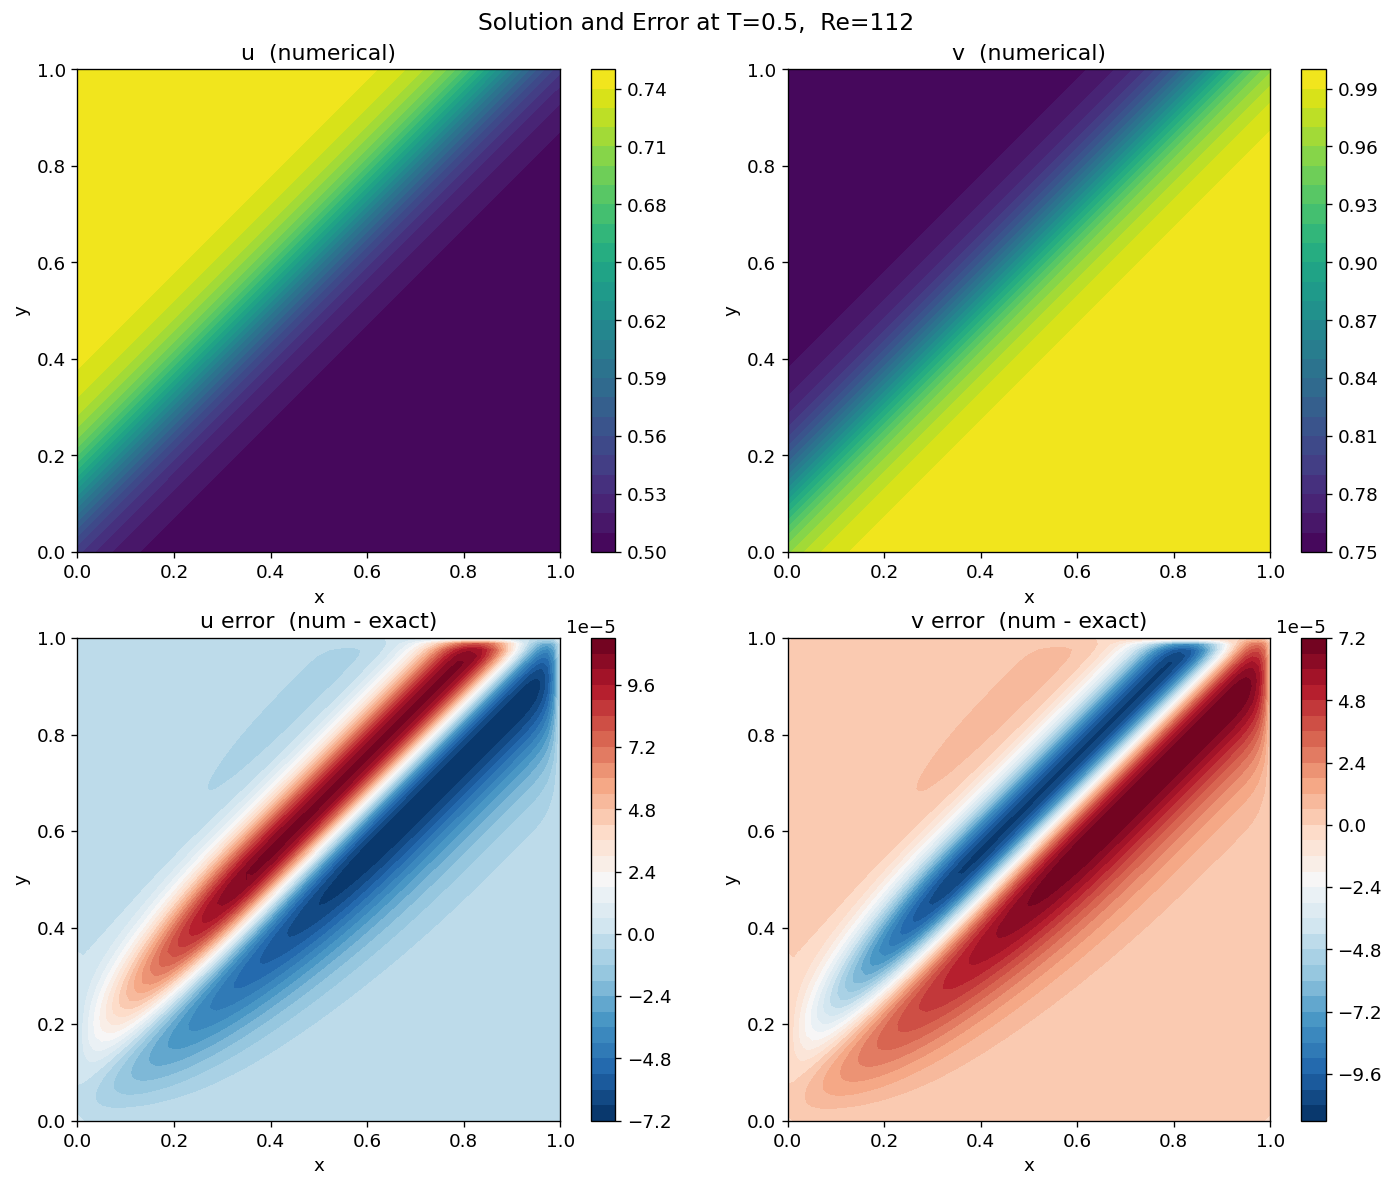
\includegraphics[width=\textwidth,height=0.42\textheight,keepaspectratio]{figures/fig_02_cell11.png}
    \end{column}
  \end{columns}
\end{frame}

% ============================================================
%  SLIDE 5 -- Spatial Convergence
% ============================================================
\begin{frame}{Spatial Convergence}
  \begin{columns}[c]
    \begin{column}{0.52\textwidth}
      \centering
      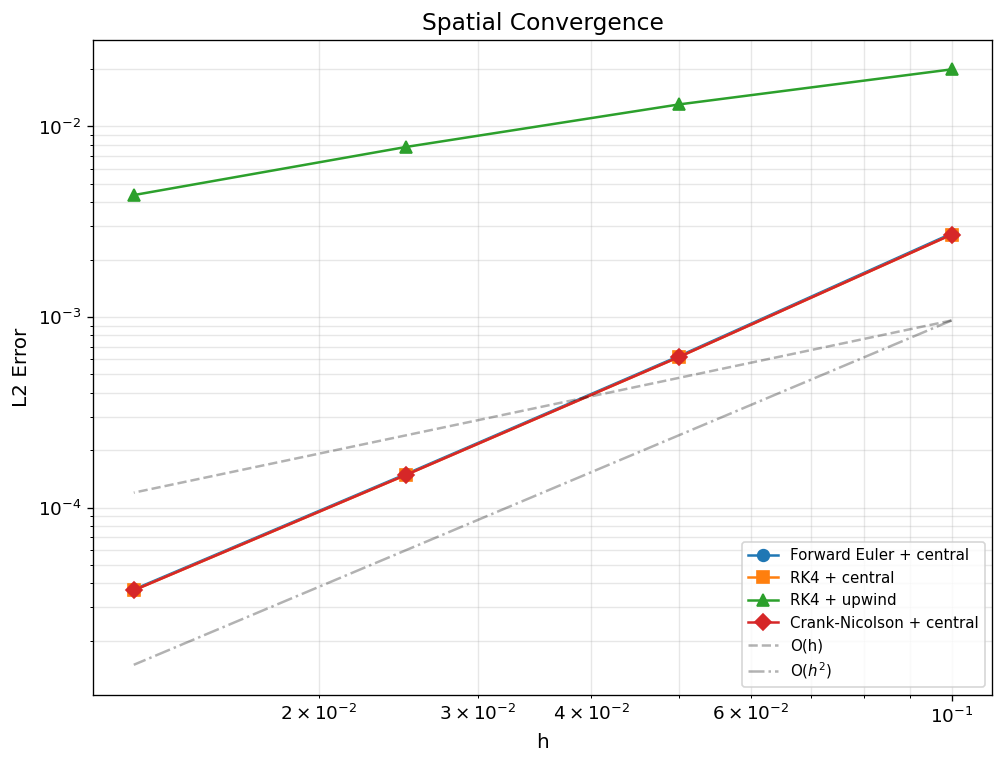
\includegraphics[width=\textwidth]{figures/fig_03_cell14.png}
    \end{column}
    \begin{column}{0.45\textwidth}
      \textbf{Key observations:}
      \begin{itemize}
        \item Central differences $\to$ $O(h^2)$ for all time integrators
        \item Upwind $\to$ $O(h)$ due to first-order spatial truncation
        \item Forward Euler, RK4, CN all collapse onto the same spatial rate when $\Delta t$ is small enough
        \item Upwind adds numerical diffusion that can mask the true solution at coarse grids
      \end{itemize}
    \end{column}
  \end{columns}
\end{frame}

% ============================================================
%  SLIDE 6 -- Temporal Convergence & Cost
% ============================================================
\begin{frame}{Temporal Convergence \& Cost vs.\ Accuracy}
  \vspace{-4pt}
  \begin{columns}[T]
    \begin{column}{0.48\textwidth}
      \centering
      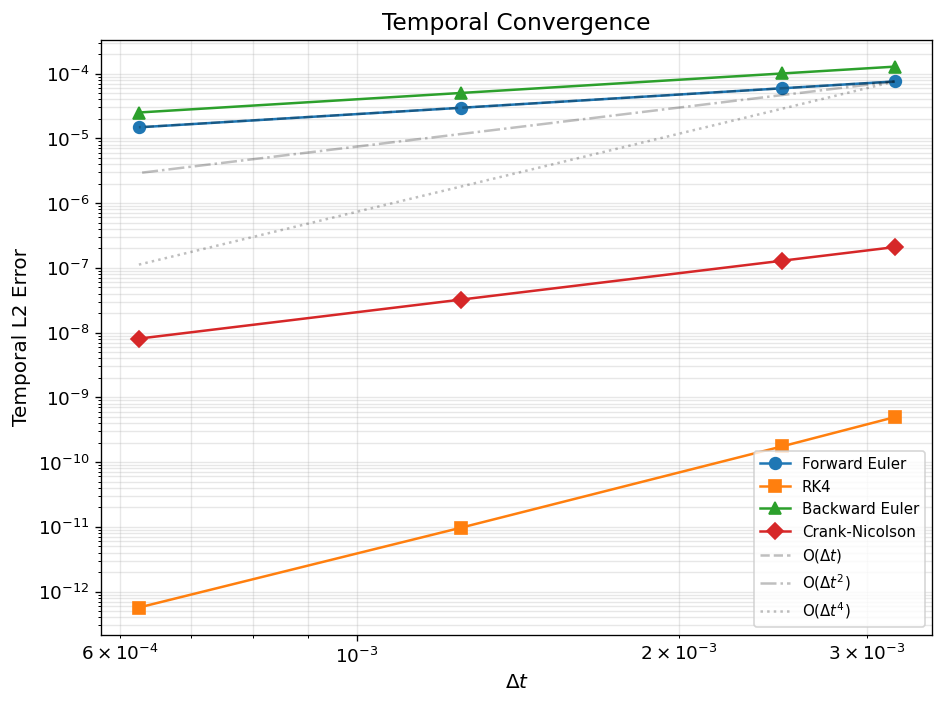
\includegraphics[width=0.95\textwidth,height=0.52\textheight,keepaspectratio]{figures/fig_04_cell17.png}
      \vspace{-4pt}
      \footnotesize
      \begin{itemize}\setlength\itemsep{1pt}
        \item FE, BE: $O(\Delta t)$\quad CN: $O(\Delta t^2)$
        \item RK4: $O(\Delta t^4)$
      \end{itemize}
    \end{column}
    \begin{column}{0.48\textwidth}
      \centering
      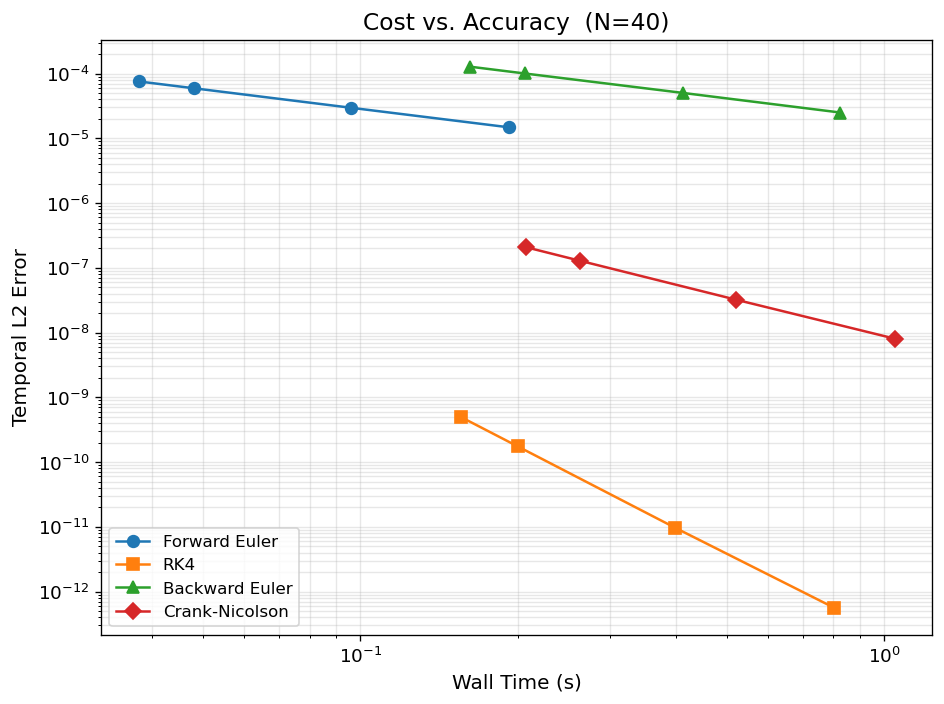
\includegraphics[width=0.95\textwidth,height=0.52\textheight,keepaspectratio]{figures/fig_05_cell19.png}
      \vspace{-4pt}
      \footnotesize
      \begin{itemize}\setlength\itemsep{1pt}
        \item RK4 reaches low error fastest
        \item Implicit methods: large $\Delta t$ but expensive per step
        \item CN: good balance at moderate accuracy
      \end{itemize}
    \end{column}
  \end{columns}
\end{frame}

% ============================================================
%  SLIDE 7 -- Stability Analysis
% ============================================================
\begin{frame}{Stability Analysis}
  \vspace{-4pt}
  \begin{columns}[T]
    \begin{column}{0.43\textwidth}
      \centering
      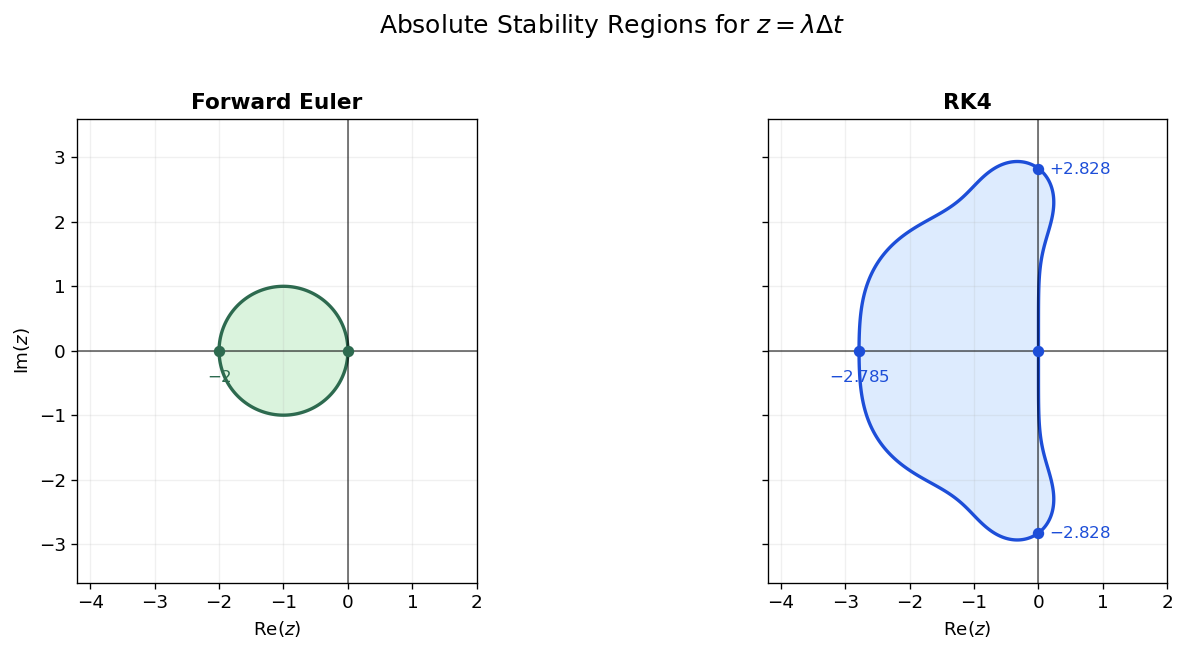
\includegraphics[width=\textwidth,height=0.48\textheight,keepaspectratio]{figures/fig_06_cell21.png}
      \vspace{-2pt}

      {\footnotesize Stability regions: FE (left), RK4 (right)}
    \end{column}
    \begin{column}{0.54\textwidth}
      \centering
      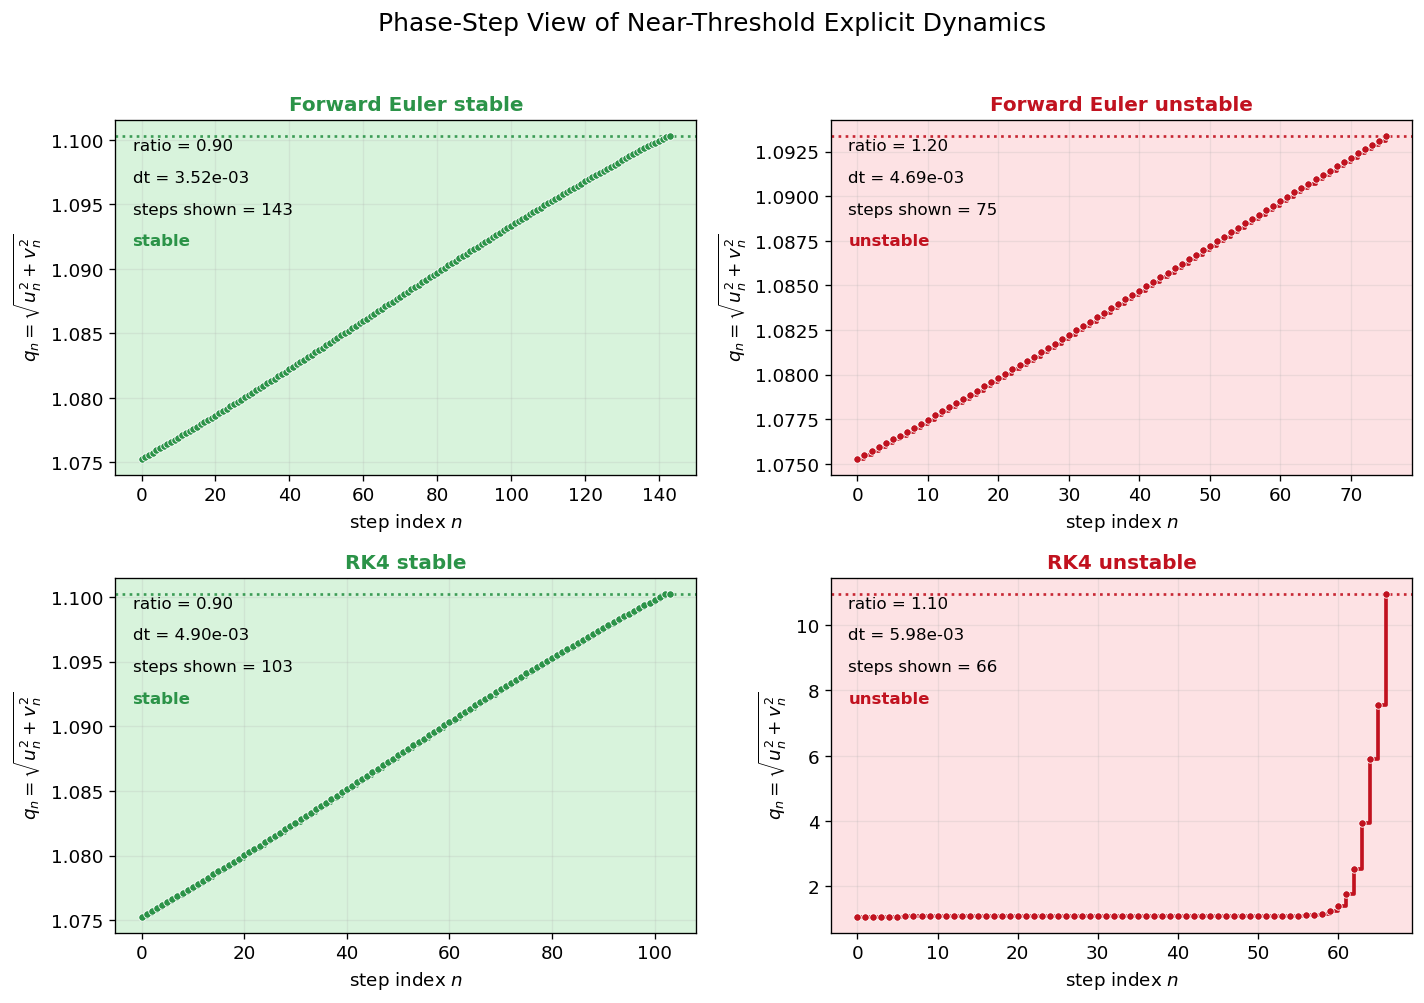
\includegraphics[width=\textwidth,height=0.48\textheight,keepaspectratio]{figures/fig_07_cell22.png}
    \end{column}
  \end{columns}

  \vspace{2pt}
  \footnotesize
  \begin{itemize}\setlength\itemsep{1pt}
    \item FE: $\Delta t \le h^2/(4\nu)$ --- very restrictive for fine grids
    \item RK4: $\approx 1.39\times$ larger stable region along the real axis
    \item Empirical probes confirm theoretical thresholds
  \end{itemize}
\end{frame}

% ============================================================
%  SLIDE 8 -- Reynolds Number Sweep
% ============================================================
\begin{frame}{Effect of Viscosity (Reynolds Number Sweep)}
  \centering
  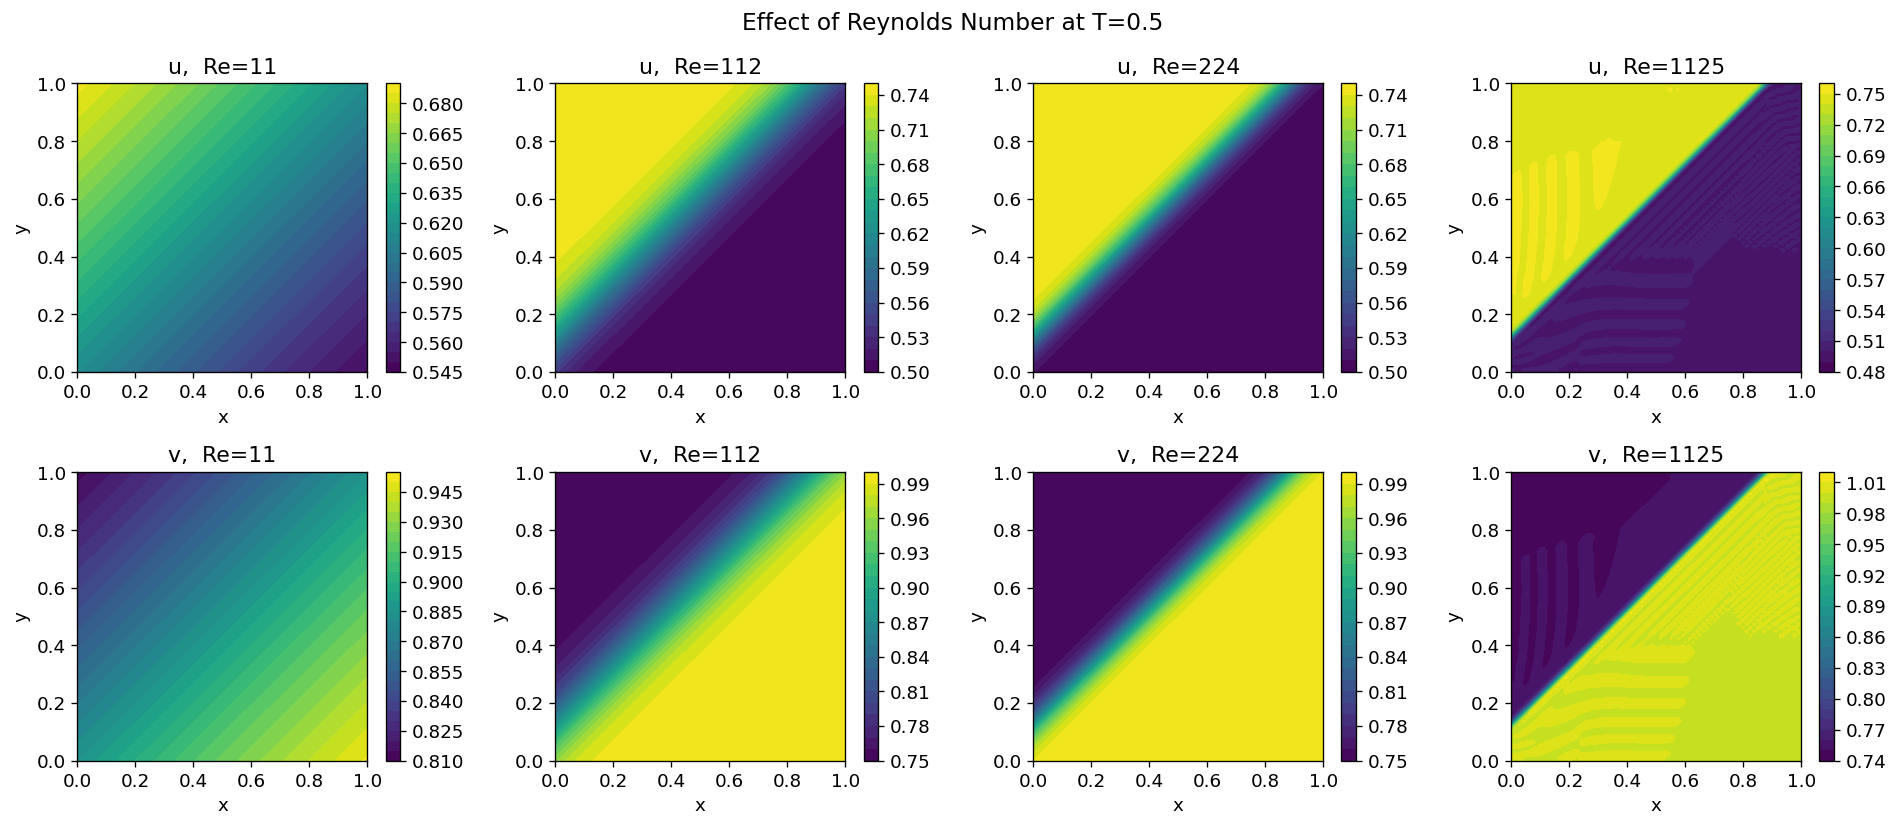
\includegraphics[width=0.82\textwidth]{figures/fig_08_cell24.png}

  \medskip
  \begin{itemize}
    \item As $\nu \to 0$ ($\mathrm{Re} \to \infty$), sharp gradients develop $\to$ finer grids or upwinding needed
    \item At $\nu = 0.001$ ($\mathrm{Re} \sim 1000$), the front resembles a shock
  \end{itemize}
\end{frame}

% ============================================================
%  SLIDE 9 -- Reflections & Future Directions
% ============================================================
\begin{frame}{Reflections \& Future Directions}
  \textbf{What we learned:}
  \begin{enumerate}
    \item Central vs.\ upwind: $O(h^2)$ accuracy vs.\ numerical diffusion trade-off
    \item Semi-implicit splitting degrades temporal order unless carefully designed (predictor-corrector CN recovers $O(\Delta t^2)$)
    \item RK4 is the most cost-effective explicit method for this problem
    \item High Re exposes the need for shock-capturing or higher-order schemes
  \end{enumerate}

  \bigskip
  \textbf{Future directions:}
  \begin{itemize}
    \item WENO / flux-limiter schemes for the advection term
    \item Adaptive mesh refinement near sharp fronts
    \item Extension to 3D or more complex nonlinear PDEs (e.g., Navier--Stokes)
    \item Multigrid or Krylov solvers for the implicit systems at scale
  \end{itemize}
\end{frame}

% ============================================================
%  SLIDE 10 -- Thank You
% ============================================================
\begin{frame}
  \centering
  \vfill
  {\Large\bfseries Thank You}

  \bigskip
  Code and notebook available in the project repository.

  \bigskip
  {\small Questions?}
  \vfill
\end{frame}

\end{document}
